\documentclass[11pt]{article}

\usepackage{comment} % enables the use of multi-line comments (\ifx \fi) 
\usepackage[a4paper,margin=1cm]{geometry}
\usepackage[utf8]{inputenc}
\usepackage[ngerman]{isodate}
\usepackage{gensymb}
\usepackage{graphicx}
\usepackage{booktabs}% http://ctan.org/pkg/booktabs
\usepackage{tabularx}
\usepackage{ltablex} % Longtables with tabularx
\usepackage[x11names]{xcolor}
\usepackage{amsmath}
\usepackage{amssymb}
\usepackage{array}
\usepackage{wrapfig}
\usepackage{subcaption}
\usepackage{csquotes}
\usepackage{lscape}
\usepackage{geometry}
\usepackage{multicol}
\usepackage{bm}
\usepackage{enumitem}
\usepackage{hyperref}
\usepackage{mdframed}
\usepackage{scalerel}
\usepackage{stackengine}
\usepackage{mathtools}
\usepackage{pdfpages}

% Code highlighting
\usepackage{minted}
\surroundwithmdframed{minted}

% Be able to caption equations and float them in place
\usepackage{float}

\newmdtheoremenv{theorem}{Theorem}
\geometry{a4paper, margin=2.4cm}

\newcommand\equalhat{\mathrel{\stackon[1.5pt]{=}{\stretchto{\scalerel*[\widthof{=}]{\wedge}{\rule{1ex}{3ex}}}{0.5ex}}}}
\newcommand\defeq{\mathrel{\overset{\makebox[0pt]{\mbox{\normalfont\tiny def}}}{=}}}
\newcolumntype{C}{>{\centering\arraybackslash}X}

\DeclarePairedDelimiter\abs{\lvert}{\rvert}
\DeclarePairedDelimiter\norm{\lVert}{\rVert}

\setcounter{tocdepth}{3}
\setcounter{secnumdepth}{3}

\graphicspath{{./img/}}

\begin{document}
	
\title{Machine Learning FS20}
\author{Pascal Baumann\\pascal.baumann@stud.hslu.ch}
\maketitle



For errors or improvement raise an issue or make a pull request on the \href{https://github.com/KilnOfTheSecondFlame/mse_summaries}{github repository}.

\tableofcontents
\newpage



\section{Introduction}

\subsection{Inductive Learning}

Inductive learning has the goal to \textbf{discover general concepts} from a \textbf{limited set of examples}, a model using inductive reasoning obtains new general knowledge from specific information. Throughout the learning process it is not truth preserving, new information can invalidate the current model, and works heuristically. The assumption therefore is that a model fitted to a sufficiently large learning set will be able to generalise to unseen data.

\begin{landscape}
	\subsubsection{Machine Learning Flowchart}
	\begin{center}
		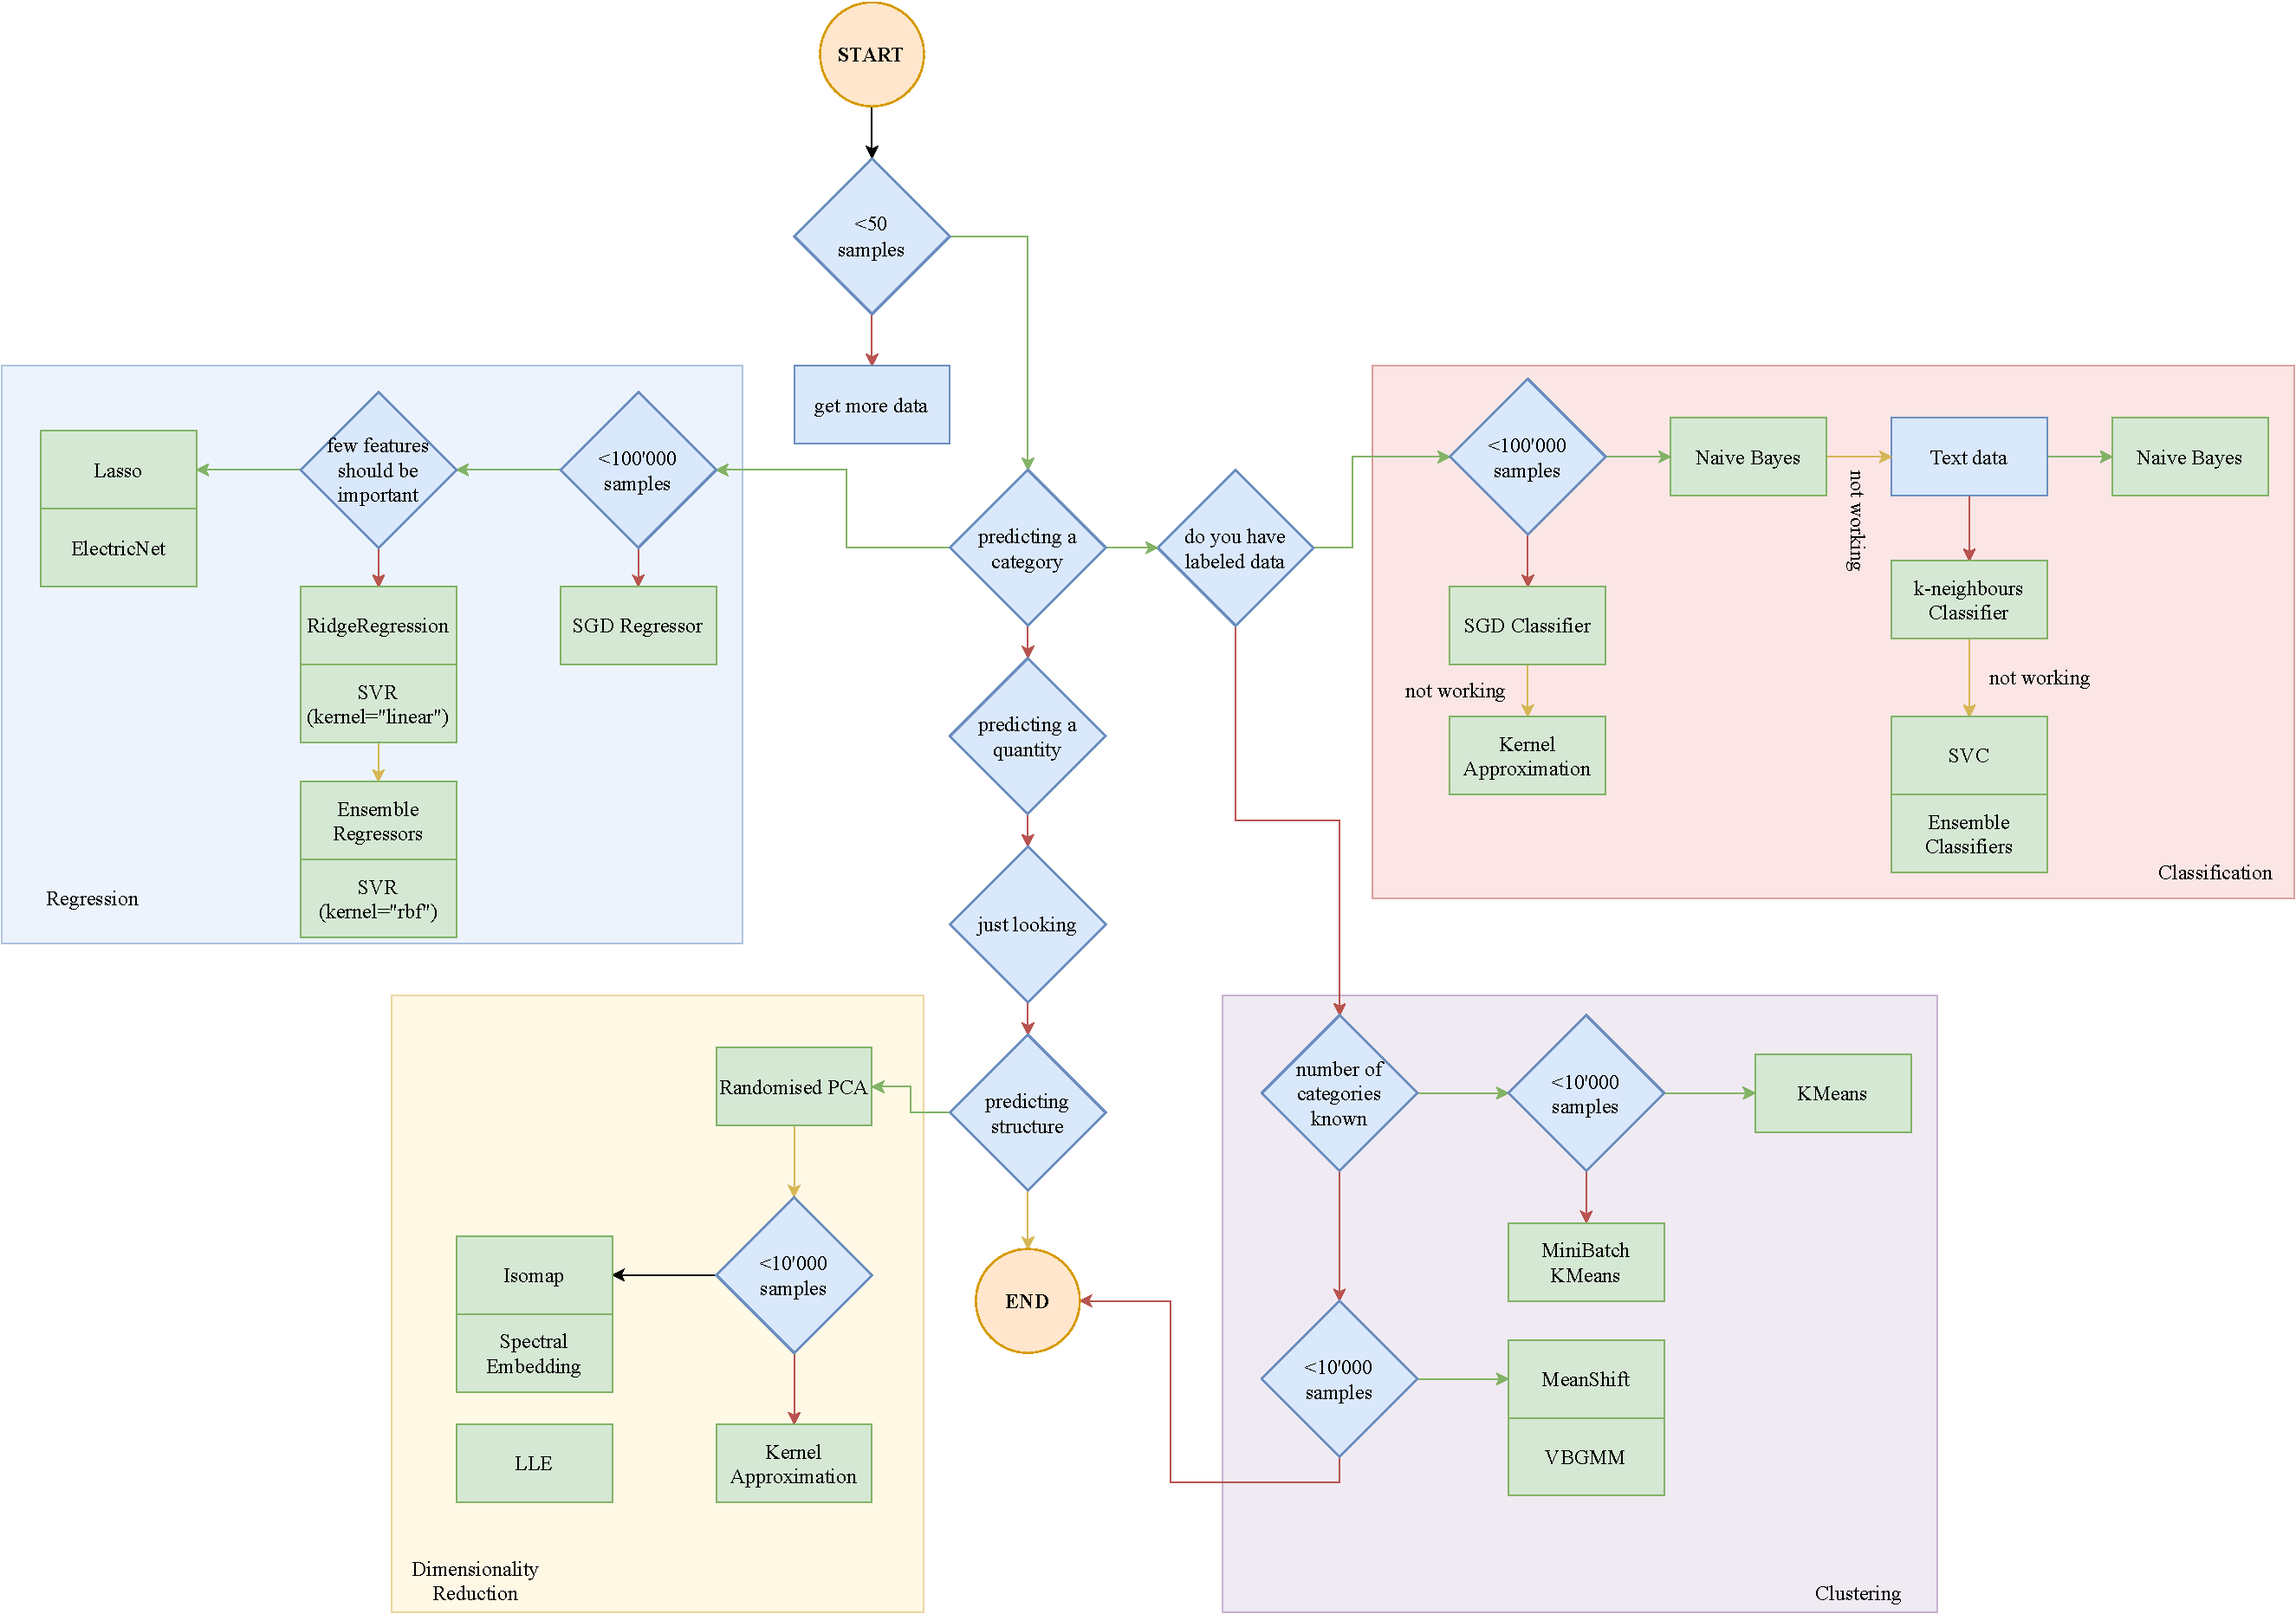
\includegraphics[height=0.9\textheight, keepaspectratio]{scikit-learn_algorithm_cheatsheet}
	\end{center}
\end{landscape}

\subsection{Inductive Supervised Learning}
The data usually has a semi-formal representation in attribute-label pairs $(\textbf{x}, y)$. The labels encode concepts or classes.
Approximate the mapping function from example $x$ to label $y$ with a hypothesis $h(x) = \hat{y} \approx f(x)$ so that it generalises well.

\subsection{Learning as Search}
\begin{center}
	\includegraphics[width=0.7\linewidth]{"../Machine Learning in Computer Visualisation/img/hypothesis_space"}
\end{center}

The hypothesis space $\mathcal{H}$ contains all possible hypotheses that can be built with the chosen representation, learning can thus be understood as a search for the global minima in this space $\mathcal{H}$.

\noindent
Formally this goal is expressed as follows: Find the hypothesis $h^* (x,\theta) = \hat{y}$ that best fits the training data, according to a loss function $L(h(x,\theta))$ by searching the hypothesis space $\mathcal{H} = \left\{ h(x,\theta) \middle| \theta \in P\right\}$.

\subsection{Inductive Bias}
\begin{theorem}
	A learner that makes \textbf{no a-priori assumptions} regarding the identity of the target concept has \textbf{no rational basis for classifying} any unseen instances. - Mitchell
\end{theorem}
All learning algorithms have some preformed hypothesis that is helpful to look for. It is beneficial to choose algorithms whose implicit hypothesis fits the data.

No free lunch theorem regarding the general equivalence of learners states that if all functions $f$ are equally likely, the probability of observing an arbitrary sequence of cost values during training does not depend on the learning algorithm $\mathcal{L}$.

The inductive bias of a learning algorithm $\mathcal{L}$ for instances in $X$ are any \textbf{minimal set of assertions} $B$ that, together with $\mathcal{L}$ and the training set $D$ \textbf{allows for deductively inferring} the $y'$ for a new $x\in X$. Make all assumptions \textbf{explicit} in $B$ such that $\forall x' \in X: \left(B, \mathcal{L}, D, x' \right) \Rightarrow y'$ is provable.

Machine Learning depends on the intelligent choice of the class $\mathcal{H}$ where $\mathcal{L}$ optimises the parameters. Machine Learning algorithms can be categorised by the strength of their inductive bias.

\subsection{Inductive Unsupervised Learning}
\begin{minipage}{0.6\linewidth}
	The usual task is Clustering, where the data $D$ are described by feature vectors without any labels, interesting structures and relationships in the data are then searched. The data naturally fall into $K$ groups, where the number of classes are not determined at the start but found through the learning scheme. This presents the challenge of searching by similarity in \textbf{distance} or \textbf{density}, which is another inductive bias to be considered, and by the choice of \textbf{parameters}.
	
\end{minipage}
\begin{minipage}{0.4\linewidth}
	\begin{center}
		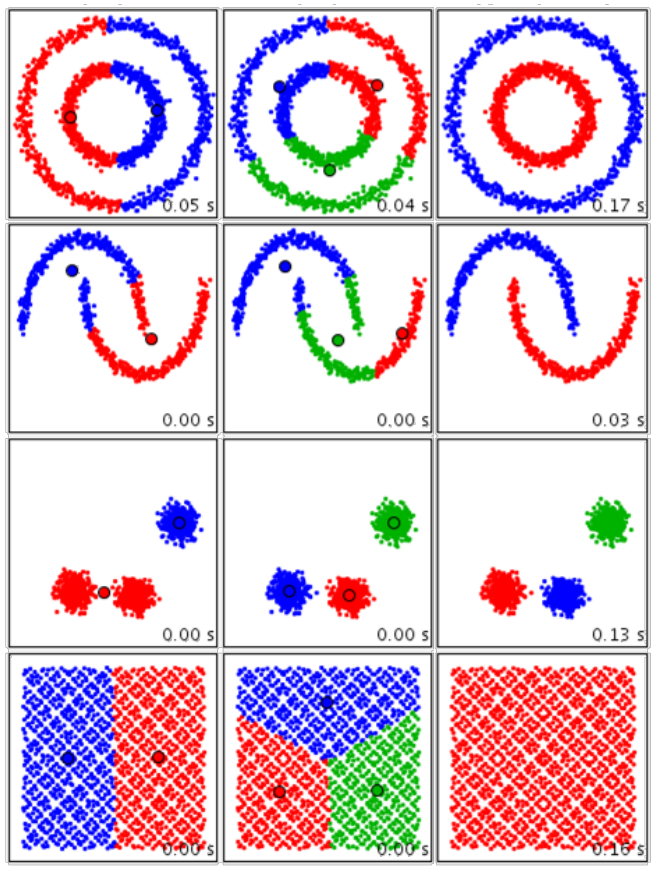
\includegraphics[width=0.6\linewidth]{img/clustering_example}
	\end{center}
\end{minipage}

\subsection{Learnability}
Any target function $f$ over an instance $X$ is learnable given an expressive enough deterministic hypothesis space $\mathcal{H}$, a large enough training set $D$, and stationarity of the distribution $X$, that is instances in $D_{\text{train}}$ and $D_{\text{test}}$ are independently, identically distributed.

Better questions are what size of \textbf{$D_{\text{train}}$} are large enough and given a large enough training set, how well does the \textbf{training error predict generalisability}. These questions are in the domain of \emph{computational learning theory}.

% TODO PAC Learnability and VC Complexity


\section{Formulating Learning Problems}
\subsection{Designing a Learning Solution}
\begin{center}
	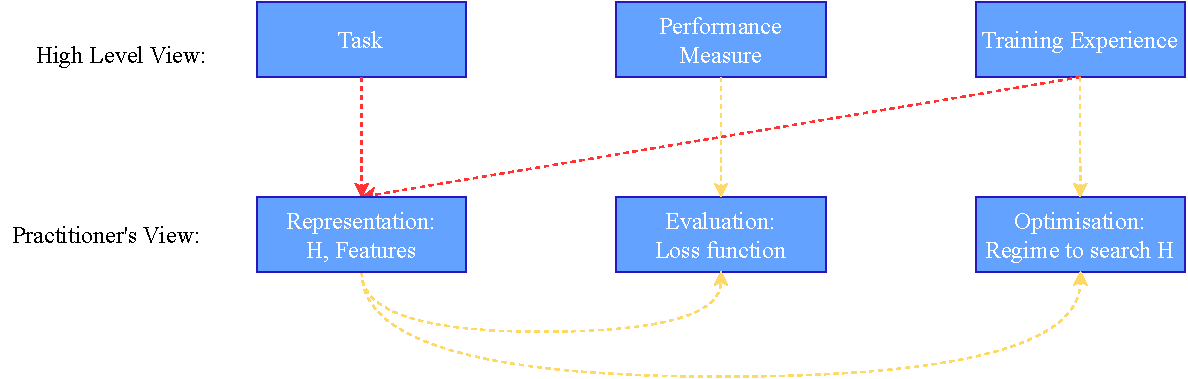
\includegraphics[width=\linewidth,keepaspectratio]{designing_learning_solution.pdf}
\end{center}

Designing a problem that is easiest for the algorithm to solve is the best thing one could do while formulating the problem. The first thing to do while first analysing data is to plot it.

\subsection{Machine Learning Development Process - Exploration and Experimentation}
There is a necessity to have a distinct conceptual approach to model data. Focus on \textbf{systematic experimentation} and \textbf{rigorous evaluation}, even automatised if needed. This is best implemented by a \textbf{pipeline of scripts} similar to the UNIX command line approach. Data exploration and rapid prototyping is key in the beginning of this process.

\begin{center}
	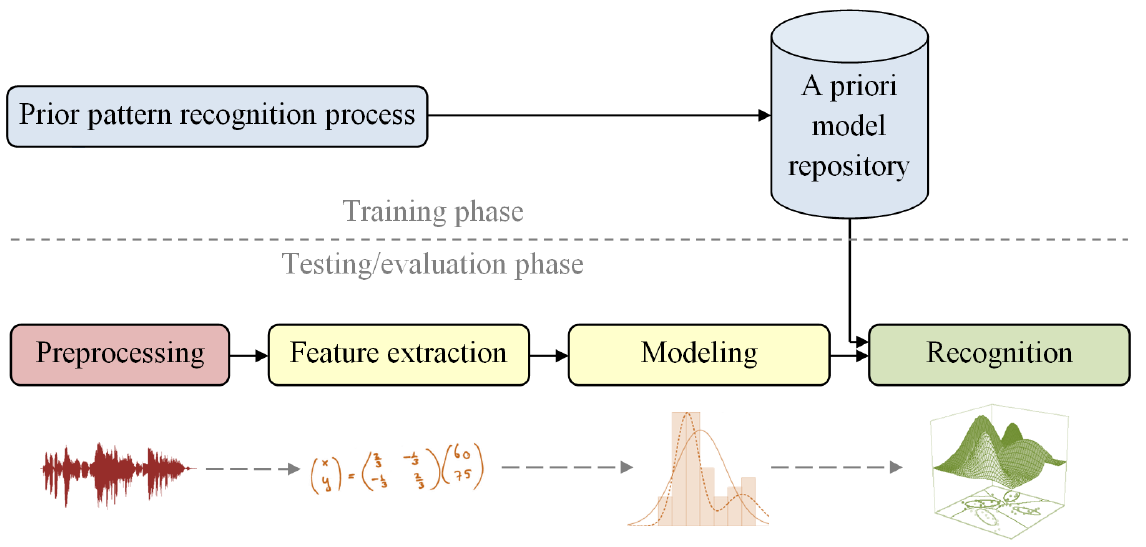
\includegraphics[width=0.6\linewidth]{exploration_evaluation_pipeline}
\end{center}

\section{Machine Learning Guiding Principles}

% TODO Cost Function $J$

% TODO Optimisation by Gradient Descent







\end{document}
